In the section \ref{sec:graphical-data-serialization-concept} the raw output from native Canvas is briefly described, while the serialized graphical data model adopted in Graphicuss system is presented in section \ref{sec:drawing-imp}. A comparison of both data model within different dimensions is performed in this part.

\subsection{Evaluation Approach}



\subsection{Dimension: Size of Canvas}



\subsection{Dimension: Amounts of Components}


\begin{figure}[!htbp]
  \centering
    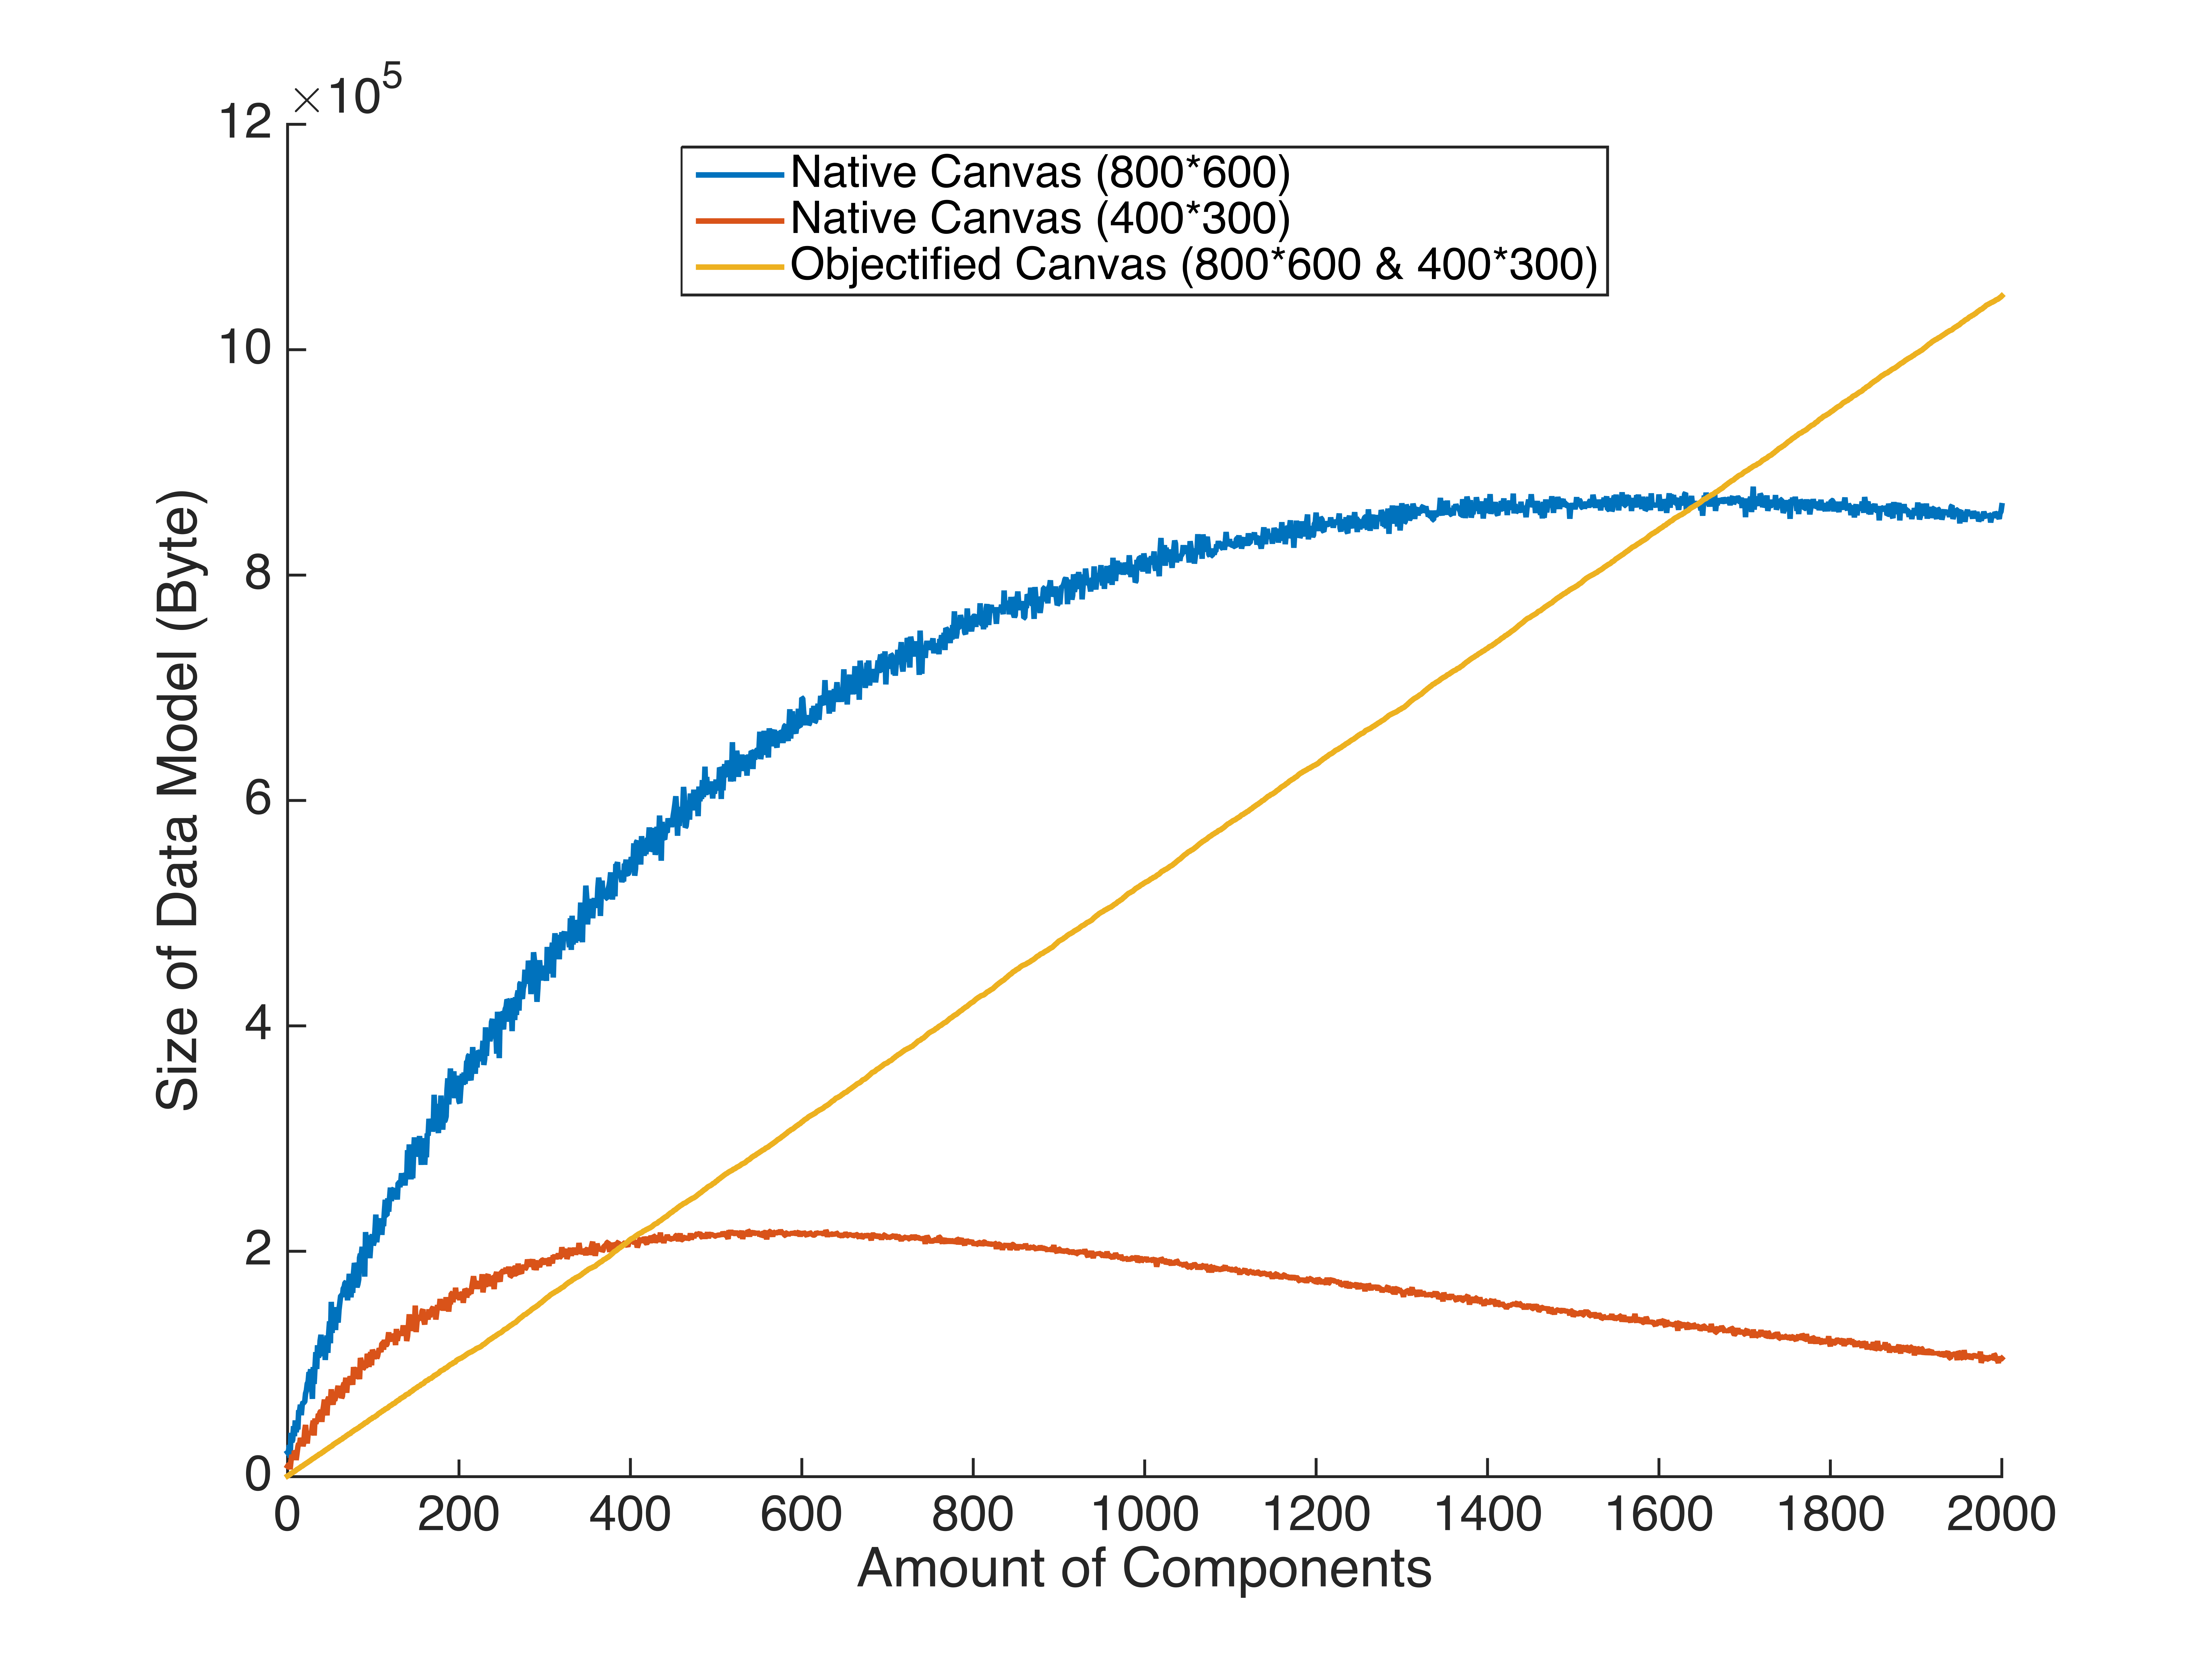
\includegraphics[width=1\textwidth]{Figures/eval-size.png}
  \caption{Comparison of data spaces of image data from native Canvas in two sizes(800*600, 400*300) and adopted graphical data model in Graphicuss}
  \label{fig:eval-nielsen}
\end{figure}